% VUT FIT MITAI
% MSZ 2021/2022
% Author: Vladimir Dusek
% Login: xdusek27

%%%%%%%%%%%%%%%%%%%%%%%%%%%%%%%%%%%%%%%%%%%%%%%%%%%%%%%%%%%%%%%%%%%%%%%%%%%%%%%%

% Path to figures
\graphicspath{{sui/strojove_uceni_generalizace/figures}}

%%%%%%%%%%%%%%%%%%%%%%%%%%%%%%%%%%%%%%%%%%%%%%%%%%%%%%%%%%%%%%%%%%%%%%%%%%%%%%%%

\chapter{SUI~--~Problém generalizace strojového učení a přístup k jeho řešení (trénovací, validační a testovací sada, regularizace, předtrénování, multi-task learning, augmentace dat, dropout, ...).}

%%%%%%%%%%%%%%%%%%%%%%%%%%%%%%%%%%%%%%%%%%%%%%%%%%%%%%%%%%%%%%%%%%%%%%%%%%%%%%%%

\section{Zdroje}

\begin{compactitem}
    \item \path{08-basics_in_ml.pdf}
    \item \path{SUI_2019-10-21.mp4}
    \item \path{SUI_2019-11-04.mp4}
    \item \path{Wikipedia}
\end{compactitem}

%%%%%%%%%%%%%%%%%%%%%%%%%%%%%%%%%%%%%%%%%%%%%%%%%%%%%%%%%%%%%%%%%%%%%%%%%%%%%%%%

\section{Strojové učení}

\begin{compactitem}
    \item Strojové učení je podoblastí umělé inteligence, zabývající se takovými algoritmy, které se dokáží samy učit -- zlepšují se na základě svých zkušeností a využívání dat, aby dosáhly vytyčeného cíle.

    \item Typicky je vytvářen (trénován, učen) model na základě trénovacích dat, který je poté schopen provádět předpovědi nebo dělat rozhodnutí, aniž by k tomu byl explicitně naprogramován.

    \item Hlavní přístupy k vytváření modelů jsou: \begin{compactitem}
        \item \textbf{Učení s učitelem} (\textit{supervised learning}) \begin{compactitem}
            \item Model je učen na označených trénovacích
            datech, která se skládají z dvojic reprezentace vstupního objektu (vektoru příznaků) a
            požadovaného výstupu.
            \item Např. klasifikace, regrese.
        \end{compactitem}

        \item \textbf{Učení bez učitele} (\textit{unsupervised learning})
        \begin{compactitem}
            \item Model je učen na neoznačených datech.
            \item Algoritmy se snaží vytvořit vhodnou a kompaktní reprezentaci vstupních dat (snížení dimenzionality, vyhlazování, diskretizace), ve které poté hledají charakteristické rysy
            a podobnosti.
            \item Např. shlukování, hledání anomálií (detekce odlehlých hodnot).
        \end{compactitem}

        \item \textbf{Zpětnovazebné učení} (\textit{reinforcement learning})
        \begin{compactitem}
            \item Model je učen na neoznačených datech ale dostává zpětnou vazbu, typicky jednou za nějaký delší časový úsek.
            \item Např. hraní her (po odehrání jedné šachové partie model dostane zpětnou vazbu, jak se mu dařilo).
        \end{compactitem}
    \end{compactitem}

    \item Trénovací algoritmy se obvykle snaží minimalizovat nějakou \textbf{chybovou funkci} (resp. objektivní funkci, \textit{objective function}), např. \begin{compactitem}
        \item MLE (\textit{Maximum likelihood estimation}) -- pro učení se pravděpodobnostních rozložení.

        \item Metoda nejmenších čtverců (\textit{Least squares}) -- pro regresi.

        \item Křížová entropie (\textit{Cross-entropy}) -- pro klasifikaci.
    \end{compactitem}

    \item Často objektivní funkce vrací chybu pro celý dataset, a chybová funkce chyby pro konkrétní datový vzorek.

    \item Komplikovanější modely (např. neuronové sítě) využívají jiné, složitější optimalizační strategie (např. gradient descent).
\end{compactitem}

%%%%%%%%%%%%%%%%%%%%%%%%%%%%%%%%%%%%%%%%%%%%%%%%%%%%%%%%%%%%%%%%%%%%%%%%%%%%%%%%

\section{Problém generalizace}

\begin{compactitem}
    \item \textbf{Generalizace} je vlastnost modelu strojového učení správně fungovat i na datech, na kterých nebyl trénován.

    \begin{compactitem}
        \item V případě klasifikace to znamená rozpoznávat co nejlépe i doposud neviděná data (data, na kterých model nebyl trénován).
    \end{compactitem}

    \item \textbf{Přetrénování} (\textit{overfitting}) -- Model se příliš specializuje na trénovací data, negeneralizuje. Trénování chceme ukončit včas, předtím, než se model začne přetrénovávat.

    \item \textbf{Podtrénování} (\textit{underfitting}) -- Model je málo natrénovaný, trénování by ještě mělo pokračovat.

    \begin{figure}[H]
        \centering
        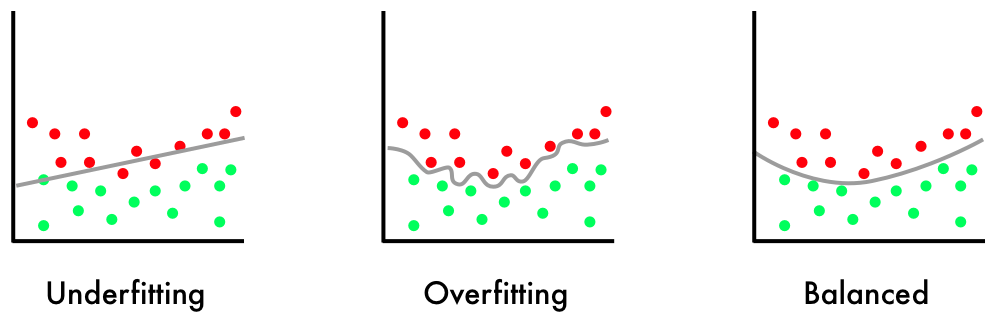
\includegraphics[width=1\linewidth]{fitting.png}
        \caption{Podtrénování, přetrování a vhodné natrénování modelu pro klasifikaci.}
    \end{figure}

    \item Jak dosáhnout toho, aby model generalizoval?
\end{compactitem}

\subsection{Rozdělení trénovací sady}

\begin{compactitem}
    \item \textbf{Trénovací sada} \begin{compactitem}
        \item Slouží k procesu trénování modelu.
        \item Typicky proces trénování opakujeme v iteracích, sledujeme hodnotu chybové funkce a upravujeme parametry modelu.
    \end{compactitem}

    \item \textbf{Validační sada} \begin{compactitem}
        \item Používá se v průběhu trénování k odhalení přetrénování modelu na trénovacích datech.
        \item Sledujeme hodnotu chybové funkce na trénovací a validační sadě. Pokud se chyba na trénovací sadě zmenšuje, ale na validační roste, model začíná být přetrénovaný.
        \item S trénovací datovou sadou je obvykle v poměru $1 : 4$.
    \end{compactitem}

    \item \textbf{Testovací sada} \begin{compactitem}
        \item Testovací sada slouží pro otestování chování modelu v reálných podmínkách, není vůbec součástí procesu trénování.
        \item Po veškerých experimentech s trénovací a validační datovou sadou je provedeno jediné vyhodnocení modelu na těchto datech.
        \item Někdy může být validační a testovací sada sjednocena a neděláme mezi něma rozdíl.
    \end{compactitem}
\end{compactitem}

\subsection{Regularizace}

\begin{compactitem}
    \item Metody jak zabránit přetrénování, a to přidáním náhodného šumu, změnou hodnot parametrů modelu (penalizace extrémních hodnot), přidání regularizačních členů do chybové funkce funkcí, \dots

    \item \textbf{Regularizace vah} \begin{compactitem}
        \item Myšlenka: můžu omezit váhy, nedopustím příliš velké hodnoty.
        \item K chybové funkci přičítám složku, která mi říká, jak moc velké jsou váhy (např. velikost vah na druhou).
    \end{compactitem}

    \item \textbf{Regularizace aktivací} \begin{compactitem}
        \item Myšlenka: můžu omezit aktivaci vrstvu.
        \item K chybové funkci přičítám složku, která mi říká, jak moc velké jsou hodnoty které vstupují do aktivační funkce.
    \end{compactitem}

    \item Formálně; $J$ je objektivní funkce, $\theta$ jsou parametry modelu, $D$ je dataset (s označenými daty -- učení s učitelem), $loss$ je chybová funkce, $f$ je model, $\lambda$ je funkce, která vrátí \uv{penalizaci} na základě velikosti vah a $\beta$ je funkce, která vrátí \uv{penalizaci} na základě velikosti aktivací.
    $$
        J(D, \theta) = \sum_{x, y}^D loss(f(x), y) + \lambda(|\theta|)^2 + \beta(|activation|)^2
    $$
\end{compactitem}

\subsection{Předtrénování}

\begin{compactitem}
    \item Způsob iniciálního nastavení parametrů modelu učení bez učitele, kdy nastavujeme parametry modelu pouze na základě vstupů na obecné datové sadě.

    \item Dotrénování následně proběhne na specifické datové sadě pomocí učení s učitelem.

    \item \textit{Nikde jsem o tomto nenašel více informací, možná to souvisí s finetuningem.}
\end{compactitem}

\subsection{Finetuning}

\begin{compactitem}
    \item Využití modelu, který byl natrénován pro podobnou úlohu a jeho dotrénování pro náš specifický problém.
    \begin{compactitem}
        \item Může být přetrénována pouze část modelu, jeho konec např.
    \end{compactitem}

    \item Využívá se typicky v neuronových sítí, např. podchytávání nějakých vzorů v obrázcích je stejné a liší se až v poslední vrstvě.

    \item Výhody: stačí menší dataset, méně výpočetního výkonu, model bude i dobře generalizovat.
\end{compactitem}

\subsection{Multi-task learning}

\begin{compactitem}
    \item Taková úloha strojového učení, ve které se řeší více učebních úloh současně, přičemž se využívají společné rysy a rozdíly mezi úlohami (model se naráz učí na několik úloh).

    \item To může vést ke zvýšení efektivity učení a přesnosti předpovědí pro modely specifické pro danou úlohu ve srovnání s tím, pokud by modely byly trénovaný odděleně.

    \item MTL zlepšuje generalizaci modelu tím, že využívá informace o doméně obsažené v tréninkových signálech příbuzných úloh jako induktivní zkreslení. Děje se tak paralelním učením úloh při použití sdílené reprezentace.

    \item V kontextu klasifikace je cílem MTL zlepšit přenost více klasifikačních úloh jejich společným učením.
    \begin{compactitem}
        \item Konkrétní příklad může být spamový filtr, který lze považovat za mnoho různých klasifikačních úloh pro každého uživatele. Různí lidé sledují různé příznaky, na základě kterých rozlišují nevyžádané e-maily od legitimních. Například anglicky mluvící člověk může zjistit, že všechny e-maily v ruštině jsou spam, u rusky mluvících lidí tomu tak není. Přesto existuje v této klasifikační úloze určitá podobnost mezi uživateli, například jedním společným rysem může být text týkající se převodu peněz. Společné řešení úlohy klasifikace spamu každého uživatele prostřednictvím MTL může umožnit, aby se řešení vzájemně informovala a zlepšila výkonnost.
    \end{compactitem}
\end{compactitem}

\subsection{Augmentace dat}

\begin{compactitem}
    \item Většina modelů strojového učení by dosáhla lepších výsledků, pokud by bylo k dispozici více trénovacích dat. Ovšem jejich získání je často poměrně nákladné.

    \item Augmentace dat je technika používaná ke zvýšení množství trénovacích dat přidáním mírně upravených kopií již existujících dat, nebo nově vytvořených syntetických vzorků z existujících dat.

    \item Typicky jde o operace: rotace, změna rozlišení, změna barev, změna kontrastu a jasu, přidání šumu, provádění výřezů, \dots
\end{compactitem}

\subsection{Dropout vrstva}

\begin{compactitem}
    \item Jde o vrstvu v neuronových sítí.

    \item Cílem je snížit náchylnost sítě k přetrénování.

    \item Spočívá v nastavení výstupu každého neuronu ve skryté vrstvě na $0$ s pravděpodobností $p$ (často $50\,\%$).

    \item K deaktivaci neuronů dochází u každého vzorku dat při trénování, do učení je tak uměle vnášen šum, díky kterému je síť schopna více generalizovat.

    \item Po ukončení trénování se síť navrátí do původního stavu a všechny váhy vedoucí z výstupu každého neuronu, resp. vstupu, se vynásobí pravděpodobností $p$, tj. pravděpodobností s jakou byl neuron ponecháván pro učení v jednotlivých minidávkách.

    \item Dropout vrstva zvýšuje počet potřebných iterací k dosažení konvergence.
\end{compactitem}
